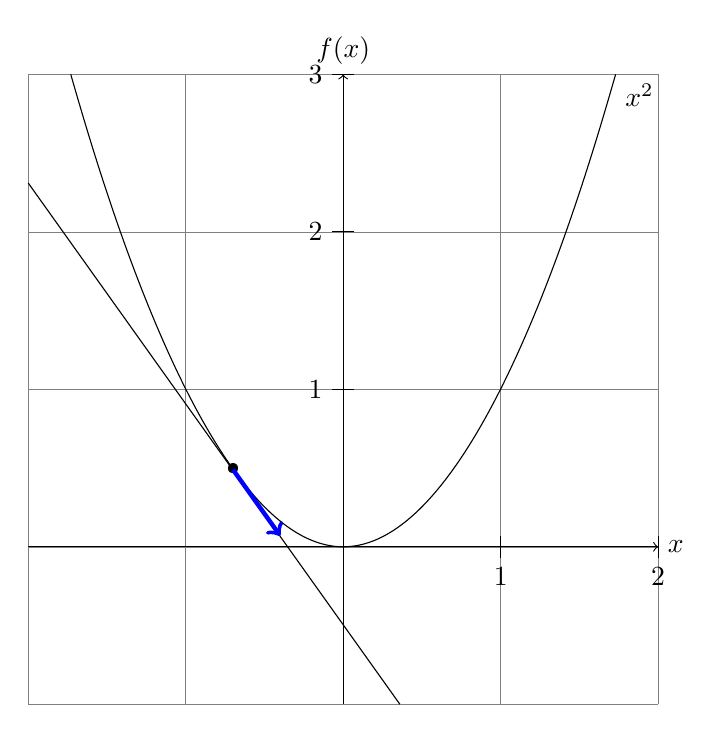
\begin{tikzpicture}[scale=2]
  \draw[style=help lines] (-2,-1) grid (2,3);

  \draw[->] (-2,0) -- (2,0) node[right] {$x$};
  \draw[->] (0,-1) -- (0,3) node[above] {$f(x)$};

  \foreach \x/\xtext in {1/1, 2/2}
    \draw[shift={(\x,0)}] (0pt,2pt) -- (0pt,-2pt) node[below] {$\xtext$};

  \foreach \y/\ytext in {1/1, 2/2, 3/3}
    \draw[shift={(0,\y)}] (2pt,0pt) -- (-2pt,0pt) node[left] {$\ytext$};

  \draw (-1.73,3) parabola bend (0,0) (1.73,3) node[below right] {$x^2$};
  \node at (-0.7, 0.49) {
    \textbullet
  };
  \draw (-2, 2.31) -- (0.36, -1);
  \draw[->, blue, ultra thick] (-0.7, 0.49) -- (-0.4, 0.07);
\end{tikzpicture}
